\section{Computational Complexity}

\subsection{Chomsky Hierarchy}
\begin{center}
    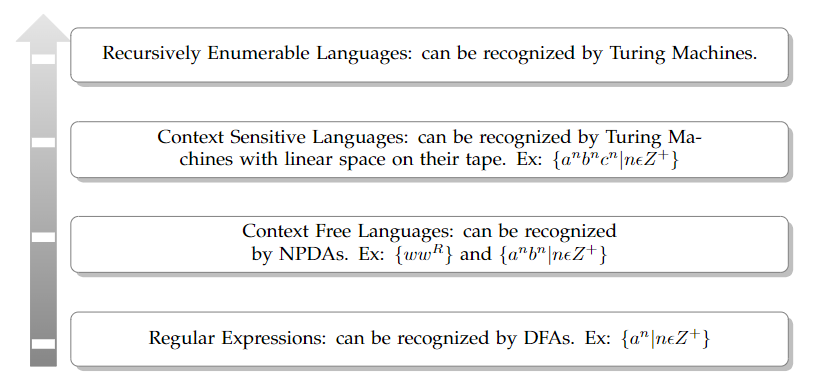
\includegraphics[scale=0.8]{figures/Chomsky_Hierarchy.png}
\end{center}
Note: a Turing Machine can ``recognize a language'' if and only if: \\
\quad TM(x) answers ``Yes'', if x is in the language, and \\
\quad TM(x) either answers ``No'' or runs forever, for all x not in the language.

\subsection{The Halting Problem}
Given a Turing Machine M and input x, we are presented with the ques-
tion: ``Does M(x) halt?'', or, \emph{does the Turing Machine give an answer instead of
running indefinitely?} The following things are true:
\begin{enumerate}
    \item Turing Machines are enumerable. Any and all Turing Machines can
    be uniquely represented by a integer. This makes sense when we con-
    sider that a binary string is a series of operations.
    \item All x's are enumerable. Turing Machines only run on integers.
    \item Universal Turing Machines exist.
\end{enumerate}

\begin{definition}
    A \emph{recursive} language is any language such that a Turing Machine
    acting on a x within the language will halt if it results in an ``Yes'' or a ``No''.
\end{definition}
\begin{definition}
    An \emph{alternating} Turing Machine is visualized as a tree that alternates 
    between levels of $\exists$ and $\forall$ with leaves that are conditional statements.
\end{definition}

\subsection{The Arithmetic Hierarchy}
$\exists =$ Existential Quantifier, or ``there exists''. \\
$\exists x: x>5$ \\
$\forall =$ Universal Quantifier, or ``for all''. \\
$\forall x : x > 5x$ \\
$\forall x \exists y : y < x - d$
\begin{center}
    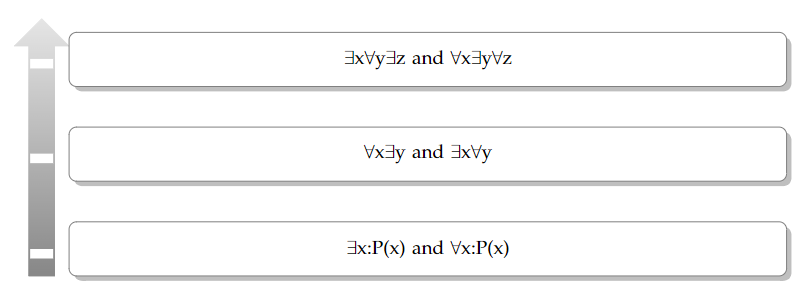
\includegraphics[scale=0.8]{figures/Arithmetic_Hierarchy.png}
\end{center}
In the lowest level of the arithmetic hierarchy $\to \exists x:P(x)$, 
$NP$ and $\forall x:P(x)$, co-$NP$. It is known that $PRIME \in$ co-NP since it is 
defined as: for all $x$, $x$ is
not an integer between 1-$n$, nor does it divide $n$. However, Pratt's Theorem
shows that $PRIME \in NP$.
\begin{theorem}
    Pratt's Theorem: $PRIME \in NP$
\end{theorem}
\begin{proof}
    If $p$ is prime, then $\Z_p^*$ is cyclic. This means that an element $g$
generates the entire group. Then, we use a non-deterministic Turing Machine
to guess $g$. To prove $g$ is a generator, for all primes that divide $p-1 =
q_1^{e_1} \cdot q_2^{e_2} \cdot \dots$, $g^{(p-1)/q_i} \not \equiv 1 (\mod p)$, 
we need only perform $\log_2 p$ tests on
primes of size and order $\log p$. We need to prove this recursively to show
that prime factors are truly prime. Thus, Pratt's Certificate of Primality requires
 the factorization of $n-1$ and the method is best applied to small
numbers (numbers $n$ known to have easily factorable $n - 1$)
\end{proof}
